\section{Propuesta de trabajo}

Como un apoyo a las personas cuya discapacidad representa un obst\'aculo para
 interactuar de manera \'agil y precisa con las computadoras de escritorio, se
 plantea desarrollar un sistema de reconocimiento de patrones con la capacidad
 reproducir las acciones que tengan mayor incidencia de uso. 
 
La propuesta presentada se enfoca utilizar una estructura de datos en
 \'arbol, en la cual se van a almacenar las acciones que el usuario realice, para
 posteriormente cuantificar las incidencias de cada rama, esto estregar\'a las
 secuencias \'utiles. Una vez detectada, se le solicitar\'a al usuario un nombre
 para esta secuencia por el cual pueda ser invocada posteriormente. 
 
En la figura~\ref{fig:arbol} se muestra un ejemplo ideal del \'arbol esperado
 despu\'es de 20 d\'ias de uso de una PC por la misma persona al realizar sus
 actividades cotidianas, donde cada camino desde el nodo ra\'iz hasta el nodo
 hoja representa las acciones realizadas por el usuario durante un d\'ia.
 
\begin{figure}[h]
\centering
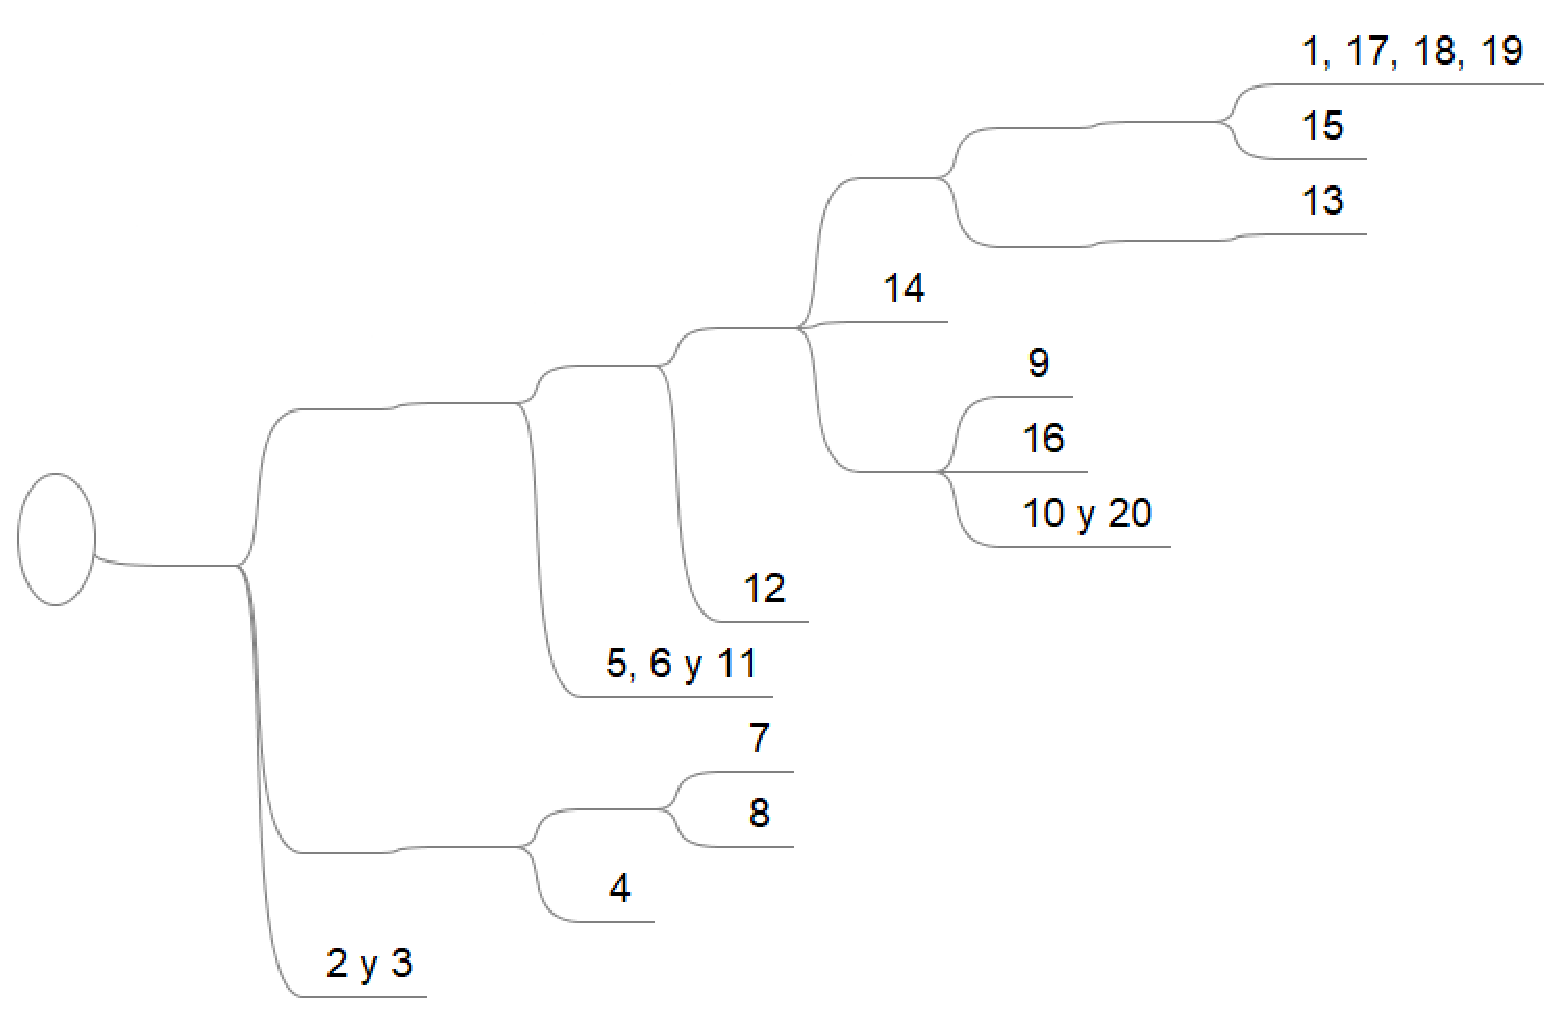
\includegraphics[width=0.8\columnwidth]{chap1/Imagenes/Arbol.eps}
\caption{Ejemplo del \'arbol ideal generado al pasar 20 d\'ias de uso de una PC.}
\label{fig:arbol}
\end{figure}